\documentclass[journal]{IEEEtran}
\usepackage[a5paper, margin=10mm]{geometry}
%\usepackage{lmodern} % Ensure lmodern is loaded for pdflatex
\usepackage{tfrupee} % Include tfrupee package


\setlength{\headheight}{1cm} % Set the height of the header box
\setlength{\headsep}{0mm}     % Set the distance between the header box and the top of the text


%\usepackage[a5paper, top=10mm, bottom=10mm, left=10mm, right=10mm]{geometry}

%
\usepackage{pythontex}
\usepackage{graphicx}
\usepackage{gensymb}
\usepackage{gvv-book}
\usepackage{gvv}
\setlength{\intextsep}{10pt} % Space between text and floats

\makeindex

\begin{document}
\bibliographystyle{IEEEtran}
\onecolumn
\section{Vector Arithmetic}
\begin{enumerate}
 \item If the coordinates of points $\vec{A}$ and $\vec{B}$ are \brak{-2,-2} and \brak{2,-4} respectively, find the coordinates of $\vec{P}$ such that $AP = \frac{3}{7} AB$, and $\vec{P}$ lies on the line segment $AB$. 
 
    \hfill {(10, 2015)}

 \solution
 Given, coordinates of $\vec{A}$ are \brak{-2,-2} and coordinates of $\vec{B}$ are \brak{2,-4}.$\vec{P}$ divides $\vec{AB}$ in ratio 3:4.So, k=$\frac{3}{4}$
 \begin{align*}
	 \implies \vec{P} &= \frac{\frac{3}{4}\vec{B} + \vec{A}}{\frac{3}{4} + 1} \\
	 &= \myvec{\frac{-2}{7}\\\frac{-20}{7}} 
 \end{align*}
          \begin{figure}
	  \begin{center}
     
		  \begin{tikzpicture}[scale=0.3,transform shape]
    \coordinate (A) at (0, 0, 0);
    \coordinate (B) at (10, 0, 0);
    \coordinate (C) at (10, 10, 0);
    \coordinate (D) at (0, 10, 0);
    \coordinate (E) at (0, 0, 10);
    \coordinate (F) at (10, 0, 10);
    \coordinate (G) at (10, 10, 10);
    \coordinate (H) at (0, 10, 10);
    
    \coordinate (P) at (5, 5, 5); 

    \draw[thick] (A) -- (B) -- (C) -- (D) -- cycle;
    \draw[thick] (E) -- (F) -- (G) -- (H) -- cycle; 
    \draw[thick] (A) -- (E);
    \draw[thick] (B) -- (F);
    \draw[thick] (C) -- (G);
    \draw[thick] (D) -- (H);
    
    \draw[dashed, thick] (A) -- (G);
    \draw[dashed, thick] (B) -- (H);

    \foreach \point in {A, B, C, D, E, F, G, H, P} {
        \filldraw[black] (\point) circle (3pt);
    }

    \node at (A) [below left] {\Huge \textbf{A}};
    \node at (B) [below right] {\Huge \textbf{B}};
    \node at (C) [above right] {\Huge \textbf{C}};
    \node at (D) [above left] {\Huge \textbf{D}};
    \node at (E) [below left] {\Huge \textbf{E}};
    \node at (F) [below right] {\Huge \textbf{F}};
    \node at (G) [above right] {\Huge \textbf{G}};
    \node at (H) [above left] {\Huge \textbf{H}};
    \node at (P) [above] {\Huge \textbf{P}};

    \draw[<->, thick] (A) -- (B) node[midway, below] {\Huge 10 m};
    \draw[<->, thick] (A) -- (D) node[midway, left] {\Huge 10 m};
    \draw[<->, thick] (E) -- (F) node[midway, below] {\Huge 10 m};

    \draw[thick] (5.5, 5.5, 4) arc[start angle=30, end angle=150, radius=1.5] node[midway, right] {\Huge $\angle GPH = \cos^{-1}\left(\frac{1}{5}\right)$};

\end{tikzpicture}


	 \end{center}	  
         \end{figure}
\end{enumerate}
\end{document}
